\section{Elliptic Curves over \texorpdfstring{$\C$}{C}}
\label{sec:over-C}

The goal of this section is to show an elliptic curve is
isomorphic to a torus as a Riemann surface.

First, let's start with the definition and some basic properties of elliptic functions.

Throughout this section, let $\Lambda \subseteq \C$ be an arbitrary lattice.

\begin{definition}
	An \emph{elliptic function} (relative to the lattice $\Lambda$) is a meromorphic function
	$f$ on $\C$, which satisfies
	\begin{equation*}
		f(z + \lambda) = f(z)\qquad\textrm{ for all } \lambda \in \Lambda, z \in \C
	\end{equation*}
\end{definition}

\begin{notation}
	The set of elliptic functions relative to the lattice $\Lambda$ is denoted
	$\C(\lambda)$.
\end{notation}

\begin{remark}
	$\C(\Lambda)$ is a field with the usual operations of 
	addition and multiplication of complex functions.
\end{remark}

\begin{definition}
	A \emph{fundamental parallelogram} for $\Lambda$ is a set of the form
	\begin{equation*}
		D = \{a + r \lambda_1 + s \lambda_2 \mid r, s \in [0, 1)\},
	\end{equation*}
	where $a \in \C$ and $\lambda_1, \lambda_2$ is a basis for $\Lambda$.
\end{definition}

\begin{proposition}
	\label{prop:no-poles}
	An elliptic function with no poles (or no zeros) is constant.
\end{proposition}

\begin{notation}
	For $f \in \C(\Lambda), z \in \C/\Lambda$, we write $f(z), \res_z(f)$ and $\ord_z(f)$ for
	$f(\bar{z}), \res_{\bar{z}}(f)$ and $\ord_{\bar{z}}(f)$ respectively,
	for any one representative
	$\bar{z} \in \C$ of the coset $z$. This is well defined by the
	$\Lambda$-periodicity of $f$.
\end{notation}

\begin{proposition}
	\label{prop:residue}
	Let $f \in \C(\Lambda)$.
	\begin{enumerate}[label=(\alph*)]
		\item $\sum_{z \in \C/\Lambda} \res_z(f) = 0$.
		\item $\sum_{z \in \C/\Lambda} \ord_z(f) = 0$.
	\end{enumerate}
\end{proposition}

Next let us introduce the Weierstrass $\wp$-function, which will serve
as a connecting link between elliptic curves and elliptic functions.

\begin{definition}
	\begin{enumerate}[label=(\alph*)]
		\item
			The Weierstrass
			elliptic function ($\wp$-function),
			is defined by the series
			\begin{equation*}
				\wp(z; \Lambda) = \frac{1}{z^2}
				+ \sum_{\lambda \in \Lambda\setminus\{0\}}
				\left(
					\frac{1}{(z-\lambda)^2} - \frac{1}{\lambda^2}
				\right)
			\end{equation*}
		\item
			The Eisenstein series (of $\Lambda$) of weight $k$,
			where $k \geq 2$ is an integer
			is the series
			\begin{equation*}
				G_k(\Lambda) = \sum_{\lambda \in \Lambda\setminus\{0\}}
				\lambda^{-k}
			\end{equation*}
	\end{enumerate}
\end{definition}

\begin{notation}
	If $\Lambda$ is known from context, we write simply
	$\wp(z)$ and $G_k$ for $\wp(z; \Lambda), G_k(\Lambda)$
	respectively.
\end{notation}

% Theorem VI.3.1
\begin{proposition}
	\label{prop:wp-properties}
	\begin{enumerate}[label=(\alph*)]
		\item	The Eisenstein series $G_k(\Lambda)$ is absolutely convergent
			for all $k \geq 3$.
		\item The series defining the Weierstrass $\wp$-function converges
			absolutely and uniformly on every compact subset of
			$\C\setminus\Lambda$. It defines a meromorphic function on $\C$ with 
			double poles of residue 0 at each lattice point.
		\item The Weierstrass $\wp$-function is an even elliptic function.
	\end{enumerate}
\end{proposition}

\begin{proof}
	\begin{enumerate}[label=(\alph*)]
	\item	Let $\lambda_1, \lambda_2$ be basis vectors of $\Lambda$.
		Let 
		\begin{equation*}
			A_N := \{n\lambda_1 + m\lambda_2 \in \Lambda \mid
			n, m \in \Z, \max(|n|, |m|) = N\}.
		\end{equation*}
		Let also 
		\begin{equation*}
			m = \min\{|a\lambda_1 + b\lambda_2| \mid 
			a, b \in \R, \max(|a|,|b|) = 1\},
		\end{equation*}
		then $m$ is well defined and strictly positive,
		as it's the minimum of a compact subset of $\R$, which does
		not contain zero. We have that
		\begin{equation*}
			\#A_N = (2N + 1)^2 - (2N - 1)^2 = 8N.
		\end{equation*}
		Furthermore, $\min\{|\lambda|, \lambda \in A_N\} \geq Nm$, so we
		get
		\begin{equation*}
			\sum_{\lambda \in \Lambda\setminus 0}\frac{1}{|\lambda|^k}
			\leq \sum_{N=1}^\infty \frac{\#A_N}{\min\{|\lambda|, \lambda \in
			A_N\}^k}
			= \sum_{N=1}^{\infty} \frac{8}{m^kN^{k-1}} < \infty.
		\end{equation*}
	\item
		If $|\lambda| > 2|z|$, then we have that
		\begin{equation*}
			|2\lambda - z| \leq 2|\lambda| + |z| \leq \frac{5}{2}|\lambda|
		\end{equation*}
		and
		\begin{equation*}
			|z - \lambda| = |\lambda|\left|\frac{z}{\lambda} - 1\right| \geq
			\frac{1}{2}|\lambda|.
		\end{equation*}
		These imply that
		\begin{equation*}
			\left| \frac{1}{(z - \lambda)^2} - \frac{1}{\lambda^2}\right|
			= \left| \frac{z(2\lambda - z)}{\lambda^2(z - \lambda)^2}\right|
			\leq 10\frac{|z|}{|\lambda|^3}
		\end{equation*}
		Hence using (a) we see that for $z \in \C \setminus \Lambda$,
		the series for $\wp(z)$ converges absolutely and uniformly on any 
		compact subset of $\C \setminus \Lambda$. It follows that
		the series defines a holomorphic function on $\C \setminus \Lambda$,
		furthermore, it is clear from the series expansion that $\wp$ has
		a double pole with residue $0$ at each point of $\Lambda$.
	\item TO BE ADDED
	\end{enumerate}
\end{proof}

\begin{theorem}
	\label{thm:wp-generates}
	We have that
	\begin{equation*}
		\C(\Lambda) = \C(\wp, \wp')
	\end{equation*}
\end{theorem}

%\begin{definition}
%	The \emph{Weierstrass $\sigma$-function} (relative to $\Lambda$) is the
%	function defined by
%	\begin{equation*}
%		\sigma(z; \Lambda) = z \prod_{\lambda\in\Lambda\setminus 0}
%		\left(1 - \frac{z}{\lambda}\right)
%		\exp\left(\frac{z}{\lambda} + \frac{1}{2}\left(\frac{z}{\lambda}\right)^2\right)
%	\end{equation*}
%\end{definition}

%\begin{notation}
%	As before, we write just $\sigma(z)$ for $\sigma(z; \Lambda)$ when $\Lambda$
%	is clear from context.
%\end{notation}

\begin{proposition}
	\label{prop:diffeq}
	For all $z \in \C \setminus \Lambda$, we have that
	\begin{equation*}
		\wp'(z)^2 = 4\wp(z)^3 - 60G_4\wp(z) - 140G_6
	\end{equation*}
\end{proposition}

\begin{remark}
	We write
	\begin{equation*}
		g_2 = g_2(\Lambda) = 60G_4
		\textrm{ and }
		g_3 = g_3(\Lambda) = 60G_3.
	\end{equation*}
	Then the equation in \ref{prop:diffeq} becomes
	\begin{equation*}
		\wp'(z)^2 = 4\wp(z)^3 - g_2\wp(z) - g_3
	\end{equation*}
\end{remark}

% Proposition VI.3.6
\begin{theorem}
	\label{thm:lattice-curve}
	Let $g_2, g_3$ be the quantities associated to $\Lambda$ as in the above
	remark.
	Let $E/\C$ be the curve given by the equation
	\begin{equation*}
		E: y^2 = 4x^3 - g_2 x - g_3
	\end{equation*}
	then $E$ is an elliptic curve and the map
	\begin{align*}
		\phi: \C/\Lambda &\to E\\
		z &\mapsto 
		\begin{cases}
			[\wp(z), \wp'(z), 1] &\textrm{if } z \not\in \Lambda\\
			[0, 1, 0] &\textrm{if } z \in \Lambda
		\end{cases}
	\end{align*}
	is a complex analytic isomorphism of complex Lie groups.
\end{theorem}

\begin{proof}
	To show $E$ is an elliptic curve, we have to show that it is non-singular.	
	From \ref{prop:singular-determinant} this is the case if and only if
	the determinant $\Delta$ of the polynomial $f(x) = 4x^3 - g_2x - g_3$
	is non-zero, in other words if and only if $f$ has no repeated roots. 
	Let $\{\lambda_1, \lambda_2\}$ be a basis of $\Lambda$,
	let $\lambda_3 = \lambda_1 + \lambda_2$. then since $\wp'$ is
	an odd elliptic function, we have that for $i \in \{1, 2, 3\}$
	\begin{equation*}
		\wp'(\lambda_i/2) = -\wp'(-\lambda_i/2) = -\wp'(\lambda_i/2)
	\end{equation*}
	and hence $\wp'(\lambda_i/2) = 0$. It follows from $\ref{prop:diffeq}$
	that $\wp(\lambda_i/2)$ is a root of $f$. So we need to show that the
	$\wp(\lambda_i/2)$ are all distinct.
	The function $\wp(z) - \wp(\lambda_i/2)$ has a double zero at $\lambda_i/2$,
	since its derivative is $\wp'(z)$ which vanishes at $\lambda_i/2$.
	Using \ref{prop:residue} and \ref{prop:wp-properties}, we deduce that these
	are the only zeroes and hence the $\wp(\lambda_i/2)$ are all distinct.
	Hence $E$ is indeed an elliptic curve.

	The image of $\phi$ is contained in $E(\C)$ by \ref{prop:diffeq}.
	Let $[x, y, 1] \in E(\C)$, then we have that $\wp(z) - x$ is a non-constant
	elliptic function, so by \ref{prop:no-poles}, it has a zero $a \in \C$.
	Hence $\wp(a) = x$ and hence by \ref{prop:diffeq}, 
	\begin{equation*}
		\wp'(a)^2 = f(\wp(a)) = f(x) = y^2.
	\end{equation*}
	It follows that $\wp'(a) = \pm y$, hence by replacing $a$ with $-a$ in
	the case $\wp'(a) =-y$, we get that $\wp'(a) = y$.
	Hence $\phi(a) = [x, y, 1]$. This shows the surjectivity of $\phi$.

	Now to show injectivity, suppose $z_1, z_2 \in \C$ are such that
	$\phi(z_1) = \phi(z_2)$. Suppose $z_1 \not\equiv -z_1 \mod \Lambda$.
	The function $\wp(z) - \wp(z_1)$ admits the roots $z_1, -z_1, z_2$, but being
	of order 2, two of these values are congruent mod $\Lambda$.
	Hence $z_2 \equiv \pm z_1 \mod \Lambda$. But since
	$\wp'(z_1) = \wp'(z_2)$, we get necessarily $z_2 \equiv z_1 \mod \lambda$.
	
	Now, if $z_1 \equiv -z_1 \mod \Lambda$, then
	\begin{equation*}
		\frac{\partial}{\partial z}(\wp(z) - \wp(z_1)) = \wp'(z)
	\end{equation*}
	and $\wp'(z_1) = \wp'(-z_1) = -\wp'(z_1)$ and hence $\wp'(z_1) = 0$.
	It follows that $z_1$ is a double root of $\wp(z) - \wp(z_1)$, which is of
	order 2. Hence $z_2$, being also a root of $\wp(z) - \wp(z_1)$, is
	necessarily congruent to $z_1$ mod $\Lambda$. This shows the injectivity
	of $\phi$.


\end{proof}

The following theorem (which we will not prove) gives the converse to \ref{thm:lattice-curve}

% Theorem VI.5.1
\begin{theorem}
	\label{thm:curve-lattice}
	Let $E/\C$ be a non-singular curve given by the equation
	\begin{equation*}
		E: y^2 = 4x^3 - ax - b.
	\end{equation*} 
	Then there exists a lattice
	$\Lambda \subseteq \C$ unique up to homothety, such that
	$a = g_2(\Lambda)$ and $b = g_3(\Lambda)$
\end{theorem}

Since any elliptic curve is isomorphic to a curve given by an equation as in
\ref{thm:curve-lattice}, we deduce that all curves are homeomorphic
to a torus $\T^2$. This allows us to calculate its homology groups.

The torus can be given a $\Delta$-complex structure
as in Figure \ref{fig:torus-delta}.
\begin{figure}[h]
	\centering 
	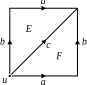
\includegraphics[width=0.4\columnwidth]{torus-delta.pdf}
	\caption[torus-delta]{$\Delta$-complex structure of a torus}
	\label{fig:torus-delta}
\end{figure}
The associated chain complex for taking simplicial homology is 
\begin{equation*}
	\begin{tikzcd}[row sep=tiny]
	\cdots & 0 & {E\Z \oplus F\Z} & {a\Z\oplus b\Z\oplus c\Z} & u\Z & 0 \\
	&&& {a,b,c} & 0 \\
	&& {E,F} & {a +b-c}
	\arrow["\partial_1", from=1-4, to=1-5]
	\arrow["\partial_2", from=1-3, to=1-4]
	\arrow[from=1-5, to=1-6]
	\arrow[from=1-2, to=1-3]
	\arrow[from=1-1, to=1-2]
	\arrow[maps to, from=3-3, to=3-4]
	\arrow[maps to, from=2-4, to=2-5]
\end{tikzcd}
\end{equation*}
Hence we get that
\begin{align*}
	H_0(\T^2) &\cong \Z,\\
	H_1(\T^2) &= \ker \partial_1 / \im \partial_2
	= a\Z \oplus b\Z \oplus c\Z / (a + b - c)\Z \cong \Z^2,\\
	H_2(\T^2) &= \ker \partial_2 = (E-F)\Z \cong \Z,
\end{align*}
and $H_n(\T^2) = 0$ for $n \geq 3$.
We deduce that the associated Betti numbers are
\begin{align*}
	b_0(\T^2) &= \rk(\Z) = 1,\\
	b_1(\T^2) &= \rk(\Z^2) = 2,\\
	b_2(\T^2) &= \rk(\Z) = 1,
\end{align*}
and $b_n(\T^2) = 0$ for $n \geq 3$.
